\section{\textcolor{unibablueI}{Time Table}}
%
\newcommand{\daywidth}{24mm}
\newcommand{\daytextwidth}{21mm}
\newcommand{\height}{4mm}
\newcommand{\oneslot}{6mm}
\newcommand{\twoslots}{13mm}
\newcommand{\threeslots}{20mm}
\newcommand{\fourslots}{27mm}
\newcommand{\fiveslots}{34mm}
\newcommand{\sixslots}{41mm}
%
\newcommand{\hourseparation}{3mm}
%
\begin{tikzpicture}[yscale=-0.1, xscale=0.1, node distance=1mm,inner sep = 0pt, outer sep = 0pt]
%
% Style for Days
\tikzstyle{day}=[white, rectangle,  minimum height=5mm, minimum width=\daywidth, fill=unibablueI,anchor=north west, align=center, font=\small]
% Style for hours
\tikzstyle{hour}=[rectangle, rounded corners, minimum height=\height, minimum width=8mm, fill=unibagrayIV, anchor=north west, align=center, font=\scriptsize]
%
\tikzstyle{default}=[anchor=north west,draw=red]
%
% Styles for events
% Duration of sequences
\tikzstyle{hours}=[rectangle,draw, minimum width=\daywidth, text width=\daytextwidth, anchor=north west, align=center, font=\footnotesize]
\tikzstyle{hhours}=[rectangle,draw, minimum width=.5*\daywidth-.5mm, text width=.5*\daytextwidth-.5mm, anchor=north west, align=center, font=\footnotesize]
%
\tikzset{grid/.style={gray,very thin,opacity=1}}
%
%\node[default] at (-7,-12) {
%        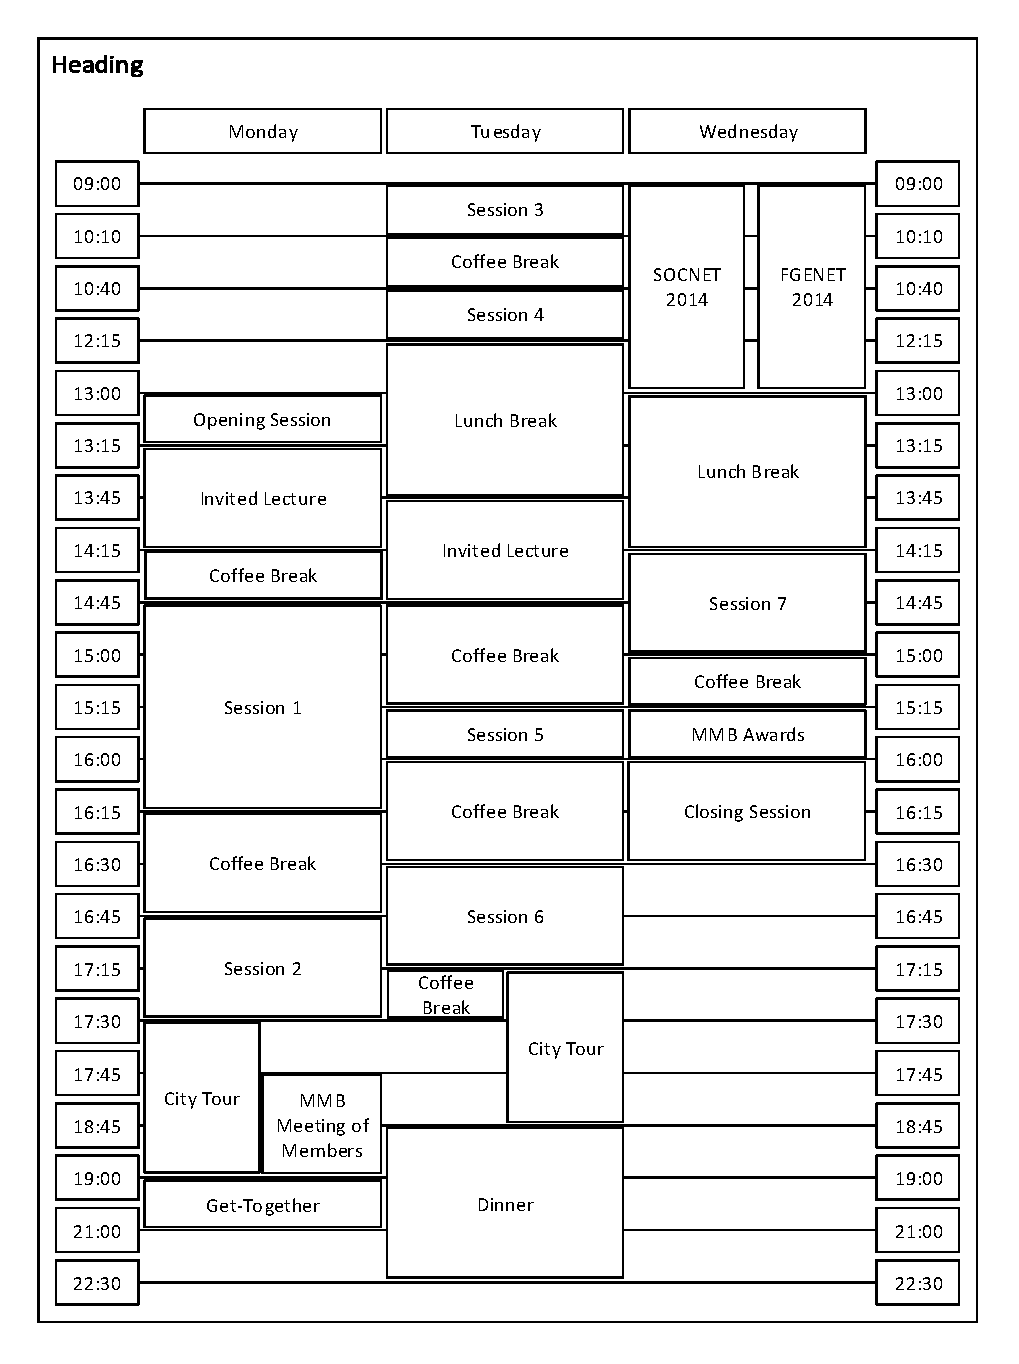
\includegraphics[width=2cm+\textwidth]{images/timetable.pdf}
%    };
%   
%\draw[grid] (0,0) grid (10*\textwidth,10*\textheight);
%
\node[day] (mo) at (9,0) {Monday};
\node[day] (tu) [right = of mo] {Tuesday};
\node[day] (we) [right = of tu] {Wednesday};
%
\node[hour] (0900) at (0,7) {09:00};
\node[hour] (1000) [below = \hourseparation of 0900] {10:00};
\node[hour] (1030) [below = \hourseparation of 1000] {10:30};
\node[hour] (1100) [below = \hourseparation of 1030] {11:00};
\node[hour] (1200) [below = \hourseparation of 1100] {12:00};
\node[hour] (1300) [below = \hourseparation of 1200] {13:00};
\node[hour] (1315) [below = \hourseparation of 1300] {13:15};
\node[hour] (1415) [below = \hourseparation of 1315] {14:15};
\node[hour] (1445) [below = \hourseparation of 1415] {14:45};
\node[hour] (1515) [below = \hourseparation of 1445] {15:15};
\node[hour] (1530) [below = \hourseparation of 1515] {15:30};
\node[hour] (1545) [below = \hourseparation of 1530] {15:45};
\node[hour] (1610) [below = \hourseparation of 1545] {16:10};
\node[hour] (1615) [below = \hourseparation of 1610] {16:15};
\node[hour] (1645) [below = \hourseparation of 1615] {16:45};
\node[hour] (1705) [below = \hourseparation of 1645] {17:05};
\node[hour] (1745) [below = \hourseparation of 1705] {17:45};
\node[hour] (1800) [below = \hourseparation of 1745] {18:00};
\node[hour] (1815) [below = \hourseparation of 1800] {18:15};
\node[hour] (1900) [below = \hourseparation of 1815] {19:00};
\node[hour] (1915) [below = \hourseparation of 1900] {19:15};
\node[hour] (2200) [below = \hourseparation of 1915] {22:00};
\node[hour] (2230) [below = \hourseparation of 2200] {22:30};
%
% Monday
\node[hhours, minimum height = \fourslots, fill=white] (reg) at($(1000.west)+(mo.north west)+(0,.5)$) {\rotatebox{90}{Registration}};
\node[hhours, minimum height = \threeslots, fill=unibagrayV] (tut) at($(1000.west)+(mo.north west)+(12.5,.5)$) {Tutorial};
\node[hours, minimum height = \oneslot, fill=white] (os) at($(1300.west)+(mo.north west)+(0,.5)$) {Opening Session};
\node[hours, minimum height = \oneslot, fill=unibayellowV] (il1) [below = of os] {\scriptsize Invited Lecture\\ S{\o}ren Asmussen};
\node[hours, minimum height = \oneslot, fill=white] (cb1) [below = of il1] {Coffee Break};
\node[hours, minimum height = \fiveslots, fill=unibablueV] (s1) [below = of cb1] {Session 1};
\node[hours, minimum height = \oneslot, fill=white] (cb2) [below = of s1] {Coffee Break};
\node[hours, minimum height = \twoslots, fill=unibablueV] (s2) [below = of cb2] {Session 2};
%% night program
\node[hhours, minimum height = \fourslots, fill=white] (ct1) at($(1745.west)+(mo.north west)+(0,.5)$) {City Tour};
\node[hhours, minimum height = \twoslots, fill=white] (mom) at($(1800.west)+(mo.north west)+(12.5,.5)$) {\scriptsize MMB Meeting of Members};
\node[hours, minimum height = \oneslot, fill=white] (gt) at($(1915.west)+(mo.north west)+(0,.5)$) {\scriptsize Welcome Reception};
%%
%% Tuesday
\node[hours, minimum height = \twoslots, fill=unibablueV] (s3) at($(0900.west)+(tu.north west)+(0,.5)$) {Session 3};
\node[hours, minimum height = \oneslot, fill=white] (cb3) [below = of s3] {Coffee Break};
\node[hours, minimum height = \twoslots, fill=unibablueV] (s4) [below = of cb3] {Session 4};
\node[hours, minimum height = \twoslots, fill=white] (lb1) [below = of s4] {Lunch Break};
\node[hours, minimum height = \twoslots, fill=unibayellowV] (il2) [below = of lb1] {Invited Lecture\\ James Roberts};
\node[hours, minimum height = \twoslots, fill=white] (cb4) [below = of il2] {Coffee Break};
\node[hours, minimum height = \threeslots, fill=unibablueV] (s5) [below = of cb4] {Session 5};
\node[hours, minimum height = \oneslot, fill=white] (cb5) [below = of s5] {Coffee Break};
\node[hours, minimum height = \twoslots, fill=unibagrayV] (s6) [below = of cb5] {Session 6};
%% night program
\node[hhours, minimum height = \twoslots, fill=white] (ct2) at($(1800.west)+(tu.north west)+(0,.5)$) {City Tour};
\node[hhours, minimum height = \oneslot, fill=white] (cb6) at($(1800.west)+(tu.north west)+(12.5,.5)$) {\scriptsize Coffee Break};
\node[hours, minimum height = \threeslots, fill=white] (di) at($(1900.west)+(tu.north west)+(0,.5)$) {Social Event};
%%
%% Wednesday
%%\node[hhours, minimum height = 31mm, fill=white] (so) at($(0900.west)+(we.north west)+(0,.5)$) {\scriptsize SOCNET 2014};
%%\node[hhours, minimum height = 31mm, fill=white] (fg) at($(0900.west)+(we.north west)+(12.5,.5)$) {\scriptsize FGENET 2014};
\node[hours, minimum height = \sixslots, fill=unibagreenV] (so) at($(0900.west)+(we.north west)+(0,.5)$) {\footnotesize Workshops\\[3ex] \footnotesize \footnotesize FGENET\\[1ex] SOCNET (-- 15:20)\\[1ex]  \footnotesize WoNeCa (-- 16:00)};
\node[hours, minimum height = \oneslot, fill=white] (lb2) at($(1315.west)+(we.north west)+(0,.5)$) {Lunch Break};
\node[hours, minimum height = \twoslots, fill=unibablueV] (s7) [below = of lb2] {Session 7};
\node[hours, minimum height = \oneslot, fill=white] (cb7) [below = of s7] {Coffee Break};
\node[hours, minimum height = \twoslots, fill=unibaredV] (ma) [below = of cb7] {MMB Awards};
\node[hours, minimum height = \oneslot, fill=white] (cs) [below = of ma] {Closing Session};
\end{tikzpicture}
\enlargethispage{3ex}